% Copyright (C) 2014-2024 by Thomas Auzinger <thomas@auzinger.name>
\let\pdfcreationdate=\creationdate
\documentclass[draft,final]{vutinfth} % Remove option 'final' to obtain debug information.

% Define convenience functions to use the author name and the thesis title in the PDF document properties.
\newcommand{\authorname}{Alexander Rinsche} % The author name without titles.
\newcommand{\thesistitle}{Context-sensitive Semantic Search in Graphs} % The title of the thesis. The English version should be used, if it exists.

% Create the XMP metadata file for the creation of PDF/A compatible documents.
\begin{filecontents*}[overwrite]{\jobname.xmpdata}
\Author{\authorname}                                    % The author's name in the document properties.
\Title{\thesistitle}                                    % The document's title in the document properties.
\Language{de-AT}                                        % The document's language in the document properties. Select 'en-US', 'en-GB', or 'de-AT'.
\Keywords{a\sep list\sep of\sep keywords}               % The document's keywords in the document properties (separated by '\sep ').
\Publisher{TU Wien}                                     % The document's publisher in the document properties.
\Subject{Thesis}                                        % The document's subject in the document properties.
\end{filecontents*}

% Load packages to allow in- and output of non-ASCII characters.
\usepackage{lmodern}        % Use an extension of the original Computer Modern font to minimize the use of bitmapped letters.
\usepackage[T1]{fontenc}    % Determines font encoding of the output. Font packages have to be included before this line.
\usepackage[utf8]{inputenc} % Determines encoding of the input. All input files have to use UTF8 encoding.

% Extended LaTeX functionality is enables by including packages with \usepackage{...}.
\usepackage{amsmath}    % Extended typesetting of mathematical expression.
\usepackage{amssymb}    % Provides a multitude of mathematical symbols.
\usepackage{mathtools}  % Further extensions of mathematical typesetting.
\usepackage{microtype}  % Small-scale typographic enhancements.
\usepackage[inline]{enumitem} % User control over the layout of lists (itemize, enumerate, description).
\usepackage{multirow}   % Allows table elements to span several rows.
\usepackage{booktabs}   % Improves the typesetting of tables.
\usepackage{subcaption} % Allows the use of subfigures and enables their referencing.
\usepackage[ruled,linesnumbered,algochapter]{algorithm2e} % Enables the writing of pseudo code.
\usepackage[dvipsnames,table]{xcolor} % Allows the definition and use of colors. This package has to be included before tikz.
\usepackage{nag}        % Issues warnings when best practices in writing LaTeX documents are violated.
\usepackage{todonotes}  % Provides tooltip-like todo notes.
\usepackage{morewrites} % Increases the number of external files that can be used.
\usepackage[a-2b,mathxmp]{pdfx}      % Enables PDF/A compliance. Loads the package hyperref and has to be included second to last.
\usepackage[acronym,toc]{glossaries} % Enables the generation of glossaries and lists of acronyms. This package has to be included last.

% Set PDF document properties
\hypersetup{
    pdfpagelayout   = TwoPageRight,           % How the document is shown in PDF viewers (optional).
    linkbordercolor = {Melon},                % The color of the borders of boxes around hyperlinks (optional).
}

\setpnumwidth{2.5em}        % Avoid overfull hboxes in the table of contents (see memoir manual).
\setsecnumdepth{subsection} % Enumerate subsections.

\nonzeroparskip             % Create space between paragraphs (optional).
\setlength{\parindent}{0pt} % Remove paragraph indentation (optional).

\makeindex      % Use an optional index.
\makeglossaries % Use an optional glossary.
%\glstocfalse   % Remove the glossaries from the table of contents.

% Set persons with 4 arguments:
%  {title before name}{name}{title after name}{gender}
%  where both titles are optional (i.e. can be given as empty brackets {}).
\setauthor{}{\authorname}{}{male}
\setadvisor{Prof.}{Emanuel Sallinger}{}{male}

% For bachelor and master theses:
\setfirstassistant{Dr.}{Eleonora Laurenza}{}{female}
%\setsecondassistant{Pretitle}{Forename Surname}{Posttitle}{male}
%\setthirdassistant{Pretitle}{Forename Surname}{Posttitle}{male}

% For dissertations:
%\setfirstreviewer{Pretitle}{Forename Surname}{Posttitle}{male}
%\setsecondreviewer{Pretitle}{Forename Surname}{Posttitle}{male}

% For dissertations at the PhD School and optionally for dissertations:
\setsecondadvisor{Pretitle}{Forename Surname}{Posttitle}{male} % Comment to remove.

% Required data.
\setregnumber{12120519}
\setdate{01}{01}{2025} % Set date with 3 arguments: {day}{month}{year}.
\settitle{\thesistitle}{Kontext-sensitive Semantische Suche in Graphen} % Sets English and German version of the title (both can be English or German). If your title contains commas, enclose it with additional curvy brackets (i.e., {{your title}}) or define it as a macro as done with \thesistitle.
\setsubtitle{Optional Subtitle of the Thesis}{Optionaler Untertitel der Arbeit} % Sets English and German version of the subtitle (both can be English or German).

% Select the thesis type: bachelor / master / doctor.
% Bachelor:
\setthesis{bachelor}
%
% Master:
%\setthesis{master}
%\setmasterdegree{dipl.} % dipl. / rer.nat. / rer.soc.oec. / master
%
% Doctor:
%\setthesis{doctor}
%\setdoctordegree{rer.soc.oec.}% rer.nat. / techn. / rer.soc.oec.

% For bachelor and master:
\setcurriculum{Software \& Information Engineering}{Software \& Information Engineering} % Sets the English and German name of the curriculum.

% Optional reviewer data:
\setfirstreviewerdata{Affiliation, Country}
\setsecondreviewerdata{Affiliation, Country}


\begin{document}

\frontmatter % Switches to roman numbering.
% The structure of the thesis has to conform to the guidelines at
%  https://informatics.tuwien.ac.at/study-services

\addtitlepage{naustrian} % German title page.
\addtitlepage{english} % English title page.
\addstatementpage

\begin{danksagung*}
Zuallererst möchte ich Prof. Emanuel Sallinger für seine fortlaufende Unterstützung, besonders aber für die initiale Unterstützung bei der Organisation der Kollaboration zwischen der TU Wien und qibri, danken. Ein besonderer Dank gebührt Tom Macdonald, welcher mich bei der Integration des Systems innerhalb der bestehenden Infrastruktur sehr unterstützt hat. Außerdem möchte ich Michael und Antonia Siegmund für die Bereitschaft diese Arbeit im Rahmen meiner Tätigkeit als Entwickler bei qibri und für die Bereitstellung notwendiger Ressourcen, danken. Abschließend möchte ich Eleonora Laurenza für ihre Beiträge und Ideen während der ersten Diskussionen und finalem Feedback danken, welche ebenfalls zur Entstehung dieser Arbeit beigetragen haben
\end{danksagung*}

\begin{acknowledgements*}
First and foremost, I would like to thank Prof. Emanuel Sallinger for his ongoing support for this thesis, especially with the initial organizational support for the collaboration between TU Wien and qibri. I am also especially grateful to Tom Macdonald, who provided continuous help in all production related matters such as deployment and hosting, when it came to setting up the system within qibri. My sincere thanks also goes to Michael and Antonia Siegmund for providing me with the opportunity as well as the resources to pursue this thesis as a part of my role as a developer at qibri. Finally, I would like to also thank Eleonora Laurenza for her contributions and ideas during the early discussions as well as some final feedback that helped shape the direction of this thesis.
\end{acknowledgements*}

\begin{kurzfassung}
Der Begriff der Semantischen Suche beschreibt das Konzept über einen Dokumentencorpus mittels Vektoren zu suchen - anstatt klassische (partial) matchings werden hierbei Suchbegriff und der Inhalt aller Dokumente mittels eines Vektorisierungs-Verfahrens in einen Vektorraum abbgebildet. Danach ist das Problem auf eine Suche nach dem/den ähnlichste(n) Vektor(en) zu dem Vektor des gewünschten Suchbegriffs reduziert. Ausschlaggebend ist hierbei, dass das Vektorisierungs-Verfahren die Domäne der Dokumente sinnvoll repräsentieren kann. Der gängige Weg ist aktuell mittels eines gewaltigen Daten- \& Rechenaufwandes diese Modele ein grobes Verständnis von Sprache zu vermitteln und dieses später aufgabenspezifisch zu verfeinern. Im Rahmen dieser Arbeit soll ein Ansatz exploriert werden, mit dem besagte aufgabenspezifische Verfeinerung dieser großen Modelle relaxiert werden kann, indem man bestehende Graphstrukturen ausnutzt, um einen ähnlichen Effekt zu erreichen. Zusätzlich wird ein System, welches aus einer Pipeline und einem fertigen Webserver zum vorbereiten und hosten einer derartigen Semantischen Suche, vorgestellt.
\end{kurzfassung}

\begin{abstract}
Semantic Search is the concept where a search over document corpus does not look for traditional word or partial word matches, but instead considers the embeddings of the query and the corpus to be searched encoded by some model. Performing a search then equates to calculating some distance metric such as euclidian distance, cosine similarity, etc. between the query embedding and all respective documents. This results in a total ordering of all documents by how similar the model evaluates the contents to the posed query. Clearly, this necessitates the model to have a decent understanding of the domain and for synonimic or otherwise related terms to achieve higher similarity scores, finetuning appears paramount, especially in corporate and technical environments with specialized langugage and vocabulary. An attempt to alleviate or at least lessen this issue will be proposed. Additionally, a semi-supervised learning pipeline to easily iterate over attempts will be proposed. Finally, a proper architecture to encapsulate this pipeline in a production-ready search engine that is easily (re-)deployable to a kubernetes cluster and can scale with demands with the necessary things in place to migrate the pipeline to an online reinforcement learning system in future work will be introduced.
\end{abstract}

% Select the language of the thesis, e.g., english or naustrian.
\selectlanguage{english}

% Add a table of contents (toc).
\tableofcontents % Starred version, i.e., \tableofcontents*, removes the self-entry.

% Switch to arabic numbering and start the enumeration of chapters in the table of content.
\mainmatter

\chapter{Introduction}

What is the definition of Information? To further specify the question, such a definition should cover the following commonly observed properties of information:
\begin{itemize}
    \item The same sentence contains a different amount of information depending on the receiver and their context
    \item It's verb ''to inform'' means to convey a fact that should influence someone's behavior.
    \item An ''informed decision'' means to be aware of as many relevant facts as possible concerning a certain decision.
\end{itemize} 
By those properties, the definition of information for this thesis will be ''facts or knowledge relevant to a receiver that influence their behavior or decisions''. The amount of information can be determined by the severity of change in their actions depending on getting or missing a said piece of information. For a machine learning model, this can essentially be measured by loss. A data sample with a high loss obviously contains more information than the last ten data samples that the model predicted correctly and therefore had little to no loss. 

From this we can draw a clear distinction between a Knowledge Base and a Information System: While a Knowledge Base is a collection of facts or, more generally speaking, knowledge, an Information System needs to actively filter the facts relevant to a user or a query.
So although a database can be considered a perfectly suitable Information System to experienced developers, for a common user there is too much (to them) uninteresting information and overhead attached to properly use it. 
For a Knowledge Base to become an Information System, a mechanism that produces the relevant information to their users at the moment where it becomes relevant, without additional overhead of filtering out unnecessary data, is paramount. In this thesis we will explore and evaluate one possible mechanism leveraging Text Embeddings and Knowledge Graph Technology.

\section{Motivation}
The recent success of transformer architectures has affected most areas of Computer Science to some degree. In the field of Information Retrieval and Search through document corpi, the technique of Semantic Search has gained new traction. While previous approaches like one hot encodings or continuous bag of words all had their shortcomings, new transformer architectures are able to capture complex relationships and meanings of words in dense vectors and through the attention mechanism that the transformer architectures all share even ambiguities of words are representable in these models.
The price is the high initial cost to train these models, the billions of parameters that need to be loaded in active memory and additional finetuning that is often required when it comes to more specialized domains.
The computational resources required for these tasks are still not accessible to most individuals and even many companies, which is why big tech companies like Google and OpenAI are currently so successful. The aim of this thesis is to lay the groundwork to propose an alternative architecture where semantic embeddings do not have to be perfect but can be improved later on without performing extensive fine-tuning of the embedding model itself and rather through exploiting additional information about the domain. Specifically, we will consider a problem statement where documents are organized in a taxonomy and form a graph structure. Optionally, individual users can also be organized and linked to taxonomy and document entities. When embedding these entities with an encoder model and using this as the initial node vectors for a Graph Neural Network, the result should yield a semantic search that is aware of a documents context and maybe even a recommendation system that can take user-based relevance into account.


\section{Data Sources}
The necessary data for training and evaluating the model was obtained from qibri.
qibri is a Knowhow Management System targeted at medium to large companies with highly specialized domain-specific knowledge. Its purpose is to manage and unify all ''Knowhow'' in a central place, to create a better overview of how well the core processes and products are documented and provide the necessary documentation to an employee when they needed. It has several mechanisms to encourage users to regularly check and update the content that they are responsible for as well as a versioning and approval process system to make sure changes are transparent, can be backtracked and are formally accepted by decision makers. Knowledge retrieval is particularly difficult in this context, however - there's a lot of information that might seem relevant when searching for a specific subject, but usually a lot of it just is not relevant to the user who started the search. So, although a document might seem to contain a lot of keywords relevant to a given search, it might still be the case that it just is not relevant due to it's particular scope and target audience within a company. To mitigate this, all documents and users are organized in a taxonomy, containing locations, departments, relevant topics, etc. The current search engine employed uses classic full text search together with logical filtering to determine if a document \textit{is} or \textit{is not} relevant to a user. However, relevance is rarely a true or false question and most recommendation systems employ sophisticated ranking mechanisms to compute an approximate ordering for the user. However, through leveraging the taxonomy qibri provides, one should be able to get a broad idea which documents are more closely related to a user's daily work and which might be less relevant, just by using the distances between them.

\section{Problem Statement}
Finding, optimizing and verifying such a system unfortunately exceeded the scope of a bachelor thesis. Therefore, the focus of this work will be on creating a sensible framework for quickly iterating over different versions. The main challenges this thesis posed were
\begin{description}
    \item[history preservation] i.e. incorporating some kind of versioning so that different extraction runs can easily be compared to each other.
    \item[extendability] building the pipeline in a way such that changes to the data extraction and the embedding process are ''easy'' to implement.
    \item[ease of deployment] - due to the classic difficulties of evaluating a recommender system or a search engine (difficulties defining ''correct'' results, relevances for different people, etc.), one of the main requirements imposed by qibri was the option to quickly deploy to production and to test it there.
\end{description}

An additional necessity that was posed by qibri was the option for logical filtering. The prior search engine, which was purely based on boolean logical filters and classical full text search, provided the user the option to filter out results based on simple logical filters such as linked taxonomies, authors and other simple true/false filters.

\subsection{Main Contributions}
The following contributions were made in the process of this thesis
\begin{itemize}
    \item \textbf{Graph Extraction Framework} A modular and expandable framework for extracting and storing a Knowledge Graph was built. Although in this case it was used specifically for the qibri application, it can easily be used for any generic extraction task. The obtained Knowledge Graph is stored in an sqlite database for ease of use in further processing. After every run a snapshot is made for ease of versioning.
    \item \textbf{Novel Semantic Contextualization Strategy} Building on the data source provided by qibri, a semantic search strategy incorporating neighborhood information into the text embeddings was proposed.
    \item \textbf{Embedding Pipeline} Using the results of the Extraction Framework, an embedding pipeline was created that can be used for obtaining semantic embeddings, or the aforementioned Semantic Contextualization strategy. This pipeline is also developed with extensibility and customizability in mind, in order to be easily adjusted to different use cases.
    \item \textbf{quaesitum Search Service} Finally, a bundled, standalone service using these building blocks was created. This service is built to handle search requests that intend to query qibris document corpus using the obtained embeddings, with ease of scaling, zero downtime reindexing and integration in a production-scale kubernetes environment in mind.
\end{itemize}
Thoroughly validating and testing the proposed strategy was unfortunately outside of the scope, as the time to be spent was already exhausted after setting up the framework and implementing a basic strategy. For further plans involving future work, refer to Chapter \ref{chap:conclusion}.


\subsection{Organization}
This thesis will be structured as follows: In Chapter \ref{chap:sentence_embeddings} and \ref{chap:graph_ml}, we introduce the necessary background for this thesis. More specifically, \ref{chap:sentence_embeddings} will focus Sentence Embeddings and Natural Language Processing, while Chapter \ref{chap:graph_ml} will give an overview over the necessary terminology and methods that enable graphs to be used in Machine Learning.
Chapter \ref{chap:methodology} will focus on the methodology applied in this thesis, the foundations and assumptions made, as well as giving an overview of the training process and how the final result can be accessed through the included webserver.
Chapter \ref{chap:discussion} focuses on the (intermediate) results and discusses potential improvements that were out of scope for this thesis. Finally, \ref{chap:conclusion} gives a quick summary of the contents of this thesis and provides an outlook of future work.


\chapter{Sentence Embeddings}\label{chap:sentence_embeddings}
This section will focus on establishing the necessary terminology and background information necessary to understand the Natural Language Processing aspects of this thesis. Particularly, a description of two distinct methods to represent text as embeddings will be provided.
\section{Word2Vec}
Representing words and, more generally speaking, text, as (relatively) low-dimensional embedding vectors (instead of the trivial method of one-hot-encoding a dictionary) such that relative distances and orientation capture some notion of meaning is one of if not the main topic of Natural Language Processing (NLP). One of the first big successes on this field was Word2Vec, which was published in a paper by Mikolov et al., at Google, in 2013. This technique uses a sliding window approach where every word in the vocabulary of the model gets projected to a dense vector and these vectors are then fit using one of two methods: \textit{Continuous bag of words} or \textit{continuous skip-gram}. Both of these methods use simple linear transformations where the one-hot-encoded word vector gets projected to a dense vector space with dimensionality $\mathcal{D}$, while the bag-of-words approach uses the surrounding to predict a missing word, the skip-gram version uses a specific input word to predict the surrounding. Figure \ref{fig:word2vec} shows a comparison between these learning approaches.
\begin{figure}
    \centering
    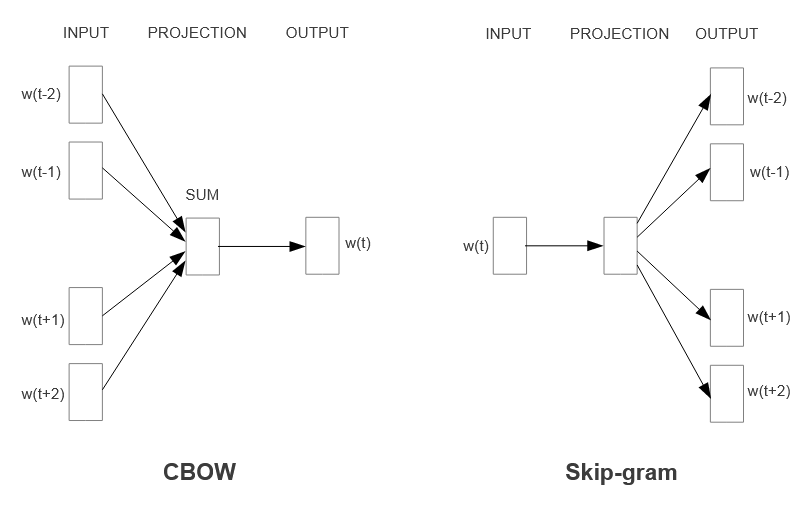
\includegraphics[width=0.9\linewidth]{thesis-figures/word2vec.png}
    \caption{Contrasting the CBOW and Skip-gram word2vec approach \cite[p. 5]{word2vec_preprint}}
    \label{fig:word2vec}
\end{figure}
The novel part of these approaches is that the predicitons are computed by another simple linear layer followed by a softmax, without any non-linearities or any larger depth. \cite{word2vec_preprint} This however suffices to learn relationships like $v('France') - v('Paris') + v('Madrid') \approx v('Spain')$, while still being quite efficient to compute. \cite{word2vec_official} The limitations arise from more complex relationships and a deeper understanding of text. By construction, Word2Vec has no mechanism to alter meaning by context, it does not even capture the sequence of words. As the term "Bag of Words" implies, the model considers no notion of ordering, words that appear before and after are summed up, averaged, and then the most similar word is predicted. The skip-gram approach also only predicts words that are also likely to appear given a specific input word, not the \textit{next} or \textit{previous} words. In addition to that, words that have several different meanings like ''bear'' or ''bow'' also are not distinguished. The semantic nuances are accumulated in a single embedding vector and any predictions are ambiguous if they were a result of the verb or the noun. A final drawback is that words that were not included in the initial vocabulary can't be assigned an embedding later on, word2vec can't assign new embeddings on the fly. With these strengths and drawbacks in mind, let's consider a more recent alternative. 


\section{The Transformer Architecture}
The paper \textit{Attention is all you need} \cite{vaswani_attention_2017} by Vaswani et al. first describes the Transformer architecture, now prominent in Large Language Models. In contrast to Word2Vec, embeddings in this architecture consist of the vector associated with the token according to the vocabulary plus a positional encoding (a combination of sine and cosine functions depending distinct for every dimension of the embedding). Additionally, although the training process bears some resemblance to the CBOW variant of Word2Vec, there are some major improvements. Instead of just predicting \textbf{a} word in a sentence based on an unordered bag consisting of previous and following words, the training process used a sequence of words as an input and the task was to predict the next word. The ''byproduct'' of this process is essentially one of the earlier versions of ChatGPT - a model that predicts what the next word (or rather token, which might also be something like a syllable) should be in a conversation repeatedly. The internal architecture to make predictions differs heavily from the initial Word2Vec model. Several components are stacked in parallel and sequentially to ensure that each word embedding incorporates the context of all of it's neighborhood (or only its predecessors, depending on the mask used). From a birds's eye view you can separate the transformer into two parts: The encoder and the decder. The encoder takes the initial input text, passes it through its network, and then passes it on to the decoder. Depending on training or inference time, the decoder either gets the target text or the generated response up until this point as an input, passes it through it's first layers, merges it together with the data received from the encoder, passes the result through the following layers and uses that to assign probabilities to all possible output-tokens to indicate their likelihood of being the next in the sequence. Figure \ref{fig:transformer-architecture} was taken from the paper by Vaswani et al. and provides a good overview of the transformer's architecture. 
\begin{figure}
    \centering
    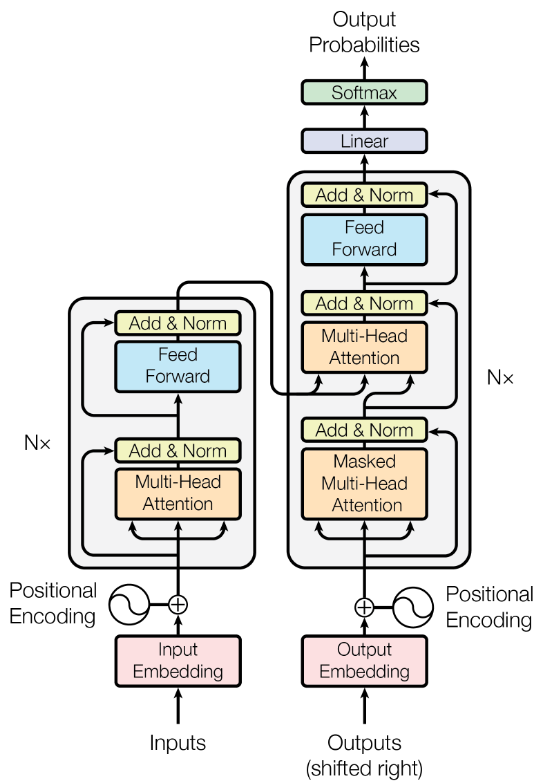
\includegraphics[width=0.6\linewidth]{thesis-figures/Transformer-Architecture.png}
    \caption{The architecture of the transformer model \cite[p. 3]{vaswani_attention_2017}}
    \label{fig:transformer-architecture}
\end{figure}As clearly illustrated by the diagram, both blocks each consist of multiple layers, the most important part, which will be briefly explained, are the \textit{self-attention}/\textit{multi-head-attention} layers. Self-attention lies of the core of incorporating the context and, as the paper title suggests, is all you need. Attention functions consist of a query and a set of key-value pairs as input, and their output is a weighted sum of the values biased by some compatibility function applied to the query and the corresponding key. This particular type of attention corresponds to this function: 
$$\mathbf{Attention}(Q,K,V) = softmax(\frac{Q \cdot K^T}{\sqrt{d_k}}) \cdot V$$
In a scenario where all of these are vectors or rather embeddings, it has an additional benefit of being easily parallelizable by using matrices instead, thereby enabling highly efficient GPU computations.\\
Self-attention is used in several different parts of a transformer. In the encoder block, it is used so that a singular word (or token) embedding incorporates the context of surrounding words and semantic connections become present. The paper even states that it appears to be benefitial to use several Self-attention layers in parallel, concatenating the results and applying a linear transformation, which suggests that there are several distinct levels of semantics that connect different parts of a text corpus (that are learned). This is called multi-head attention. Figure \ref{fig:paying-attention} shows a graphic illustration of both attention mechanisms
\begin{figure}
    \centering
    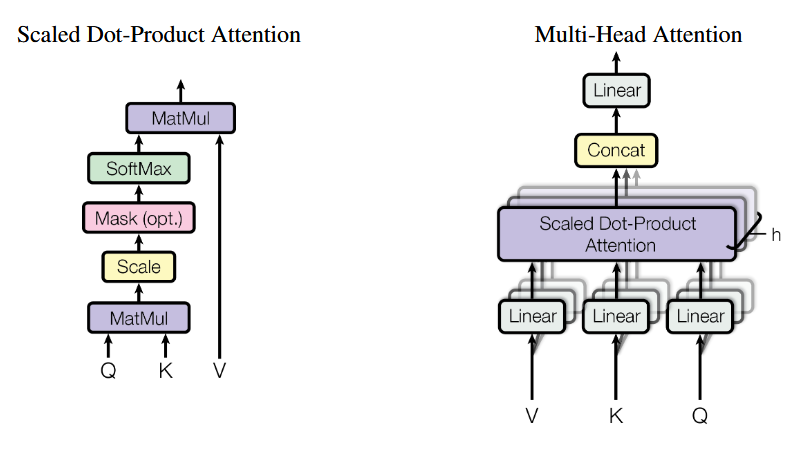
\includegraphics[width=1.0\linewidth]{thesis-figures/Attention.png}
    \caption{Self-attention (left) and Multi-Head Attention (right) \cite[p. 4]{vaswani_attention_2017}}
    \label{fig:paying-attention}
\end{figure}
The next use in the architecture is in the first layers of the decoder stack. The idea is the same as in the encoder, however, every word embedding is only allowed to use its \textbf{predecessors} as context, following embeddings are masked out. This is to ensure that the model learns to predict the next word in the output and does not use information present only in the training as an unwanted shortcut. The final use of an attention layer lies in the mergeing of encoder and decoder stacks. In this case  the question posed is ''Which parts of the input are related to which parts of the output''. Or, in terms of the paper ''This allows every position in the decoder to attend over all positions in the input sequence.'' \cite[p. 5]{vaswani_attention_2017}

\section{Obtaining embeddings from Transformers}
The final step in the ladder regarding Text embeddings that will be briefly explained, is BERT, which stands for Bidirectional Encoder Representations from Transformers. While the initial transformers purpose was purely generative in nature, BERT is more a jack-of-all-trades type of model. It's used for tasks such as question answering where it finds the answer to a question within a given paragraph, sentiment analysis, classifying inferences between two sentences, semantic similarities and many more. There are several new concepts it introduced: Fully bidirectional attention mechanisms without masking - while the initial Transformer architecture by Vaswani et al. suggested Masking in the self-attention layers to prevent ''cheating'', BERT only uses masks in the actual training data, there is no masking in the entire architecture. This enables word embeddings to attend to the entire context, not only predecessors or successors. The way this is achieved is by altering the (pre-)training task - instead of predicting the next token, parts of the input are randomly masked and the task of the model is to predict the initial token which was supposed to be there. Additionally, the paper demonstrated how a single pretrained BERT instance can easily be finetuned to several different tasks - and outperformed many task-specific architectures at the time. The general architecture is identical to the encoder stack of the initial transformer architecture discussed previously. An input can be a single piece of text, or two connected halves, which are tokenized by a vocabulary that is built up of likelihood-based word and subword fragments with WordPiece \cite{wu_googles_2016} and then fed through the neural network. A special addition is a starting token ($\mathtt{[CLS]}$), which is prepended to each statement. This can then used for classification tasks later on. The $\mathtt{[SEP]}$ token is used to split the input into two segments, for tasks like quesion answer pairs and sentence inference. 
\begin{figure}[h!]
    \centering
    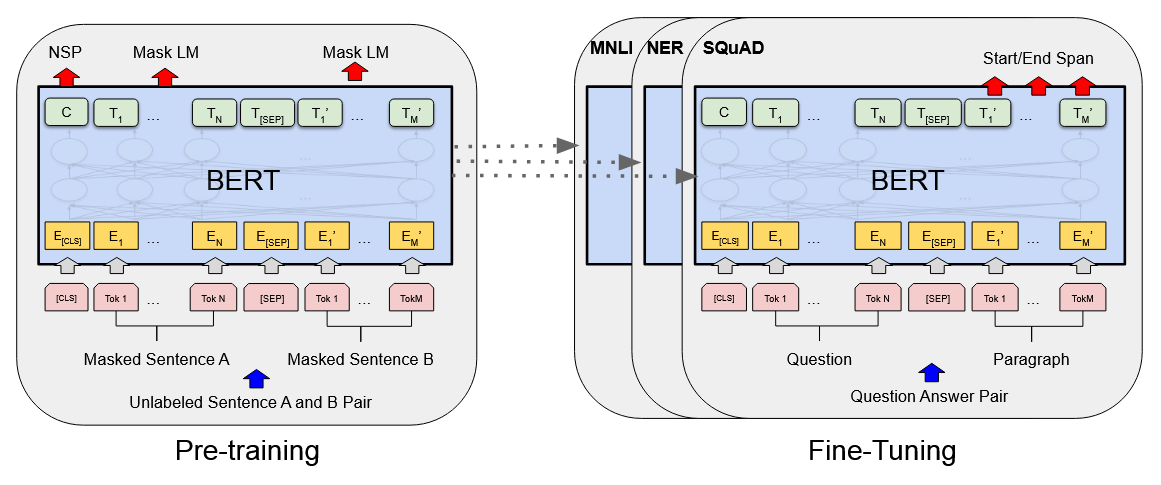
\includegraphics[width=0.9\linewidth]{thesis-figures/BERT-Architecture.png}
    \caption{Overview over the training process of a BERT model. \cite[p. 4173]{BERT}}
    \label{fig:BERT-training-setup}
\end{figure}


Figure \ref{fig:BERT-training-setup} illustrates the training process with a single pre-training and any arbitrary amount of fine-tuning for task specific heads. The output of the neural network is a set of text embeddings for each token of the input with context information from all other tokens. These are what can then be used for the previously mentioned downstream tasks. The pre-training consists of the aforementioned masking, dubbed ''Masked Language Model'' or MLM for short, and Next Sentence Prediction (NSP). For NSP, the model gets two sentences and has to predict if the second one follows the first in the original text corpus, or if it is a non-connected random sentence. For this task, the embedding of the $\mathtt{[CLS]}$ token at the beginning of the sequence is used. \cite{BERT}

\chapter{Graphs in Machine Learning} \label{chap:graph_ml}
This chapter focuses on the graph-specific aspects of this thesis. The terminology of a Knowledge Graph will be briefly discussed, followed by a characterization of Graph Neural Networks and the description of one particular popular example, GraphSAGE.


\section{Knowledge Graphs}
A Knowledge Graph (KG) can formally be described as a set of triples of the form 
$\mathtt{< head,\ relation,\ tail>}$. The ''Knowledge'' part from a Knowledge Graph is that each part of a triple is supposed to reference some sort of real-world entity or concept. Therefore each reference has some sort notion of semantics with additional \textit{Knowledge} attached, which can be explicitly or implicitly modeled in the Knowledge Graph. Instances of Knowledge Graphs include (but are not limited to) the financial domain \cite{Bellomarini_Magnanimi_Nissl_Sallinger_2021}, where ownership, trade and similar relations form the links between people, companies or even entire countries, the bio-medical domain \cite{Lu_Goi_Zhao_Wang_2025}, where molecular structures, proteins etc. are used to model interactions and likelihoods of diseases, toxins and other substances relevant to modern medicine, and many more.

There are several benefits from using Knowledge Graphs to model your domain. Firstly, the aforementioned data model is very simple and can be represented in all kinds of data stores (not limited to graph stores!). Additionally, it's a powerful abstraction that enables sophisticated reasoning over a simple interface while still being able to tap into all the underlying complexity at will. Finally, there are well-established methodologies from the fields of reasoning and inference as well as machine learning, which are easily applicable to KGs. From the reasoning/database disciplines, there are tools such as Datalog, Answer Set Programming and Ontology-based reasoning such as the Semantic Web Stack with OWL and RDF. As for machine learning, models such as Knowlege Graph Embeddings (KGEs) and Graph Neural Networks (GNNs) are prime examples. GNNs will be further discussed in the next section, as they are a key part of this thesis. KGEs are a model that tries to map a set of triples (and thereby a Knowledge Graph) in a vector domain, where the nodes (which are represented by the heads and tails of the triples) are represented as points in this domain and relations are some sort of operation or formula for a pair of nodes to determine if the model predicts there to be an edge between the two or not. A classic example from literature is TransE, where relations are simple offset vectors and an edge is predicted as true iff the following equation holds true: $$embed(\mathtt{head}) + embed(\mathtt{relation}) \approx embed(\mathtt{tail})$$ 
The reason why this is not well-suited for this thesis is that KGEs \textit{only} learn the graph structure and features of nodes (and edges) are generally not incorporated into the model's embeddings. Additionally, KGE's tend to struggle with dynamic graphs and local upgrades.


\section{Graph Neural Networks}
In this section the general concept of a Graph Neural network (GNN) will be explored, followed by a more in-depth exploration of two specific models, Graph Convolutional Neural Networks (GCNs) and GraphSAGE.
A Graph Neural Network is a special type of a Multi-Layer Perceptron which is well established in Machine Learning. As the name implies, its intended for graph structures, which make it an important tool for to leverage Knowledge Graphs. The basic concept is that of a message passing network, where each node carries certain information (represented as a feature vector), which it's neighbors can see and have access to and let it influence their own feature vectors. Repeating this accumulation of data from the neighborhood and allowing it to bias a node's feature vector means more and more general structural information from further distances will accumulate in the individual nodes. A general equation that captures this notion of aggregating and adjusting that (almost) all GNNs share is the following:
$$h^{n+1}_i = \delta(h^n_i,AGG(\{h^n_j | v_j \in \mathcal{N}_{v_i}\}))$$
$h^n_i$ represents the feature vector of vertex $v_i$ after $n$ iterations, $\delta$ and $AGG$ are activation and aggregation functions that differ between models and can contain learnable parameters and finally $\mathcal{N}_{v_i}$ is the set of vertices adjacent to $v_i$ (with no clear order). Note that this means $AGG$ takes an \textit{unordered} sequence of nodes as an input and has to be permutation-independent function. 
Their applications range from recommender systems (which will be a focus of this thesis), over social networks, traffic prediction, financial and biological applications to Computer Vision and text classification problems. Needless to say, they are a very powerful tool with a variety of applications. \cite{Explainable_GNNs} Figure \ref{fig:GNN-pipeline} shows a high-level overview to the pipeline of a GNN. The input for this thesis is the extracted graph consisting of users, documents and taxonomy elements and the features are text embeddings of the content for every node.
\begin{figure}[h!]
    \centering
    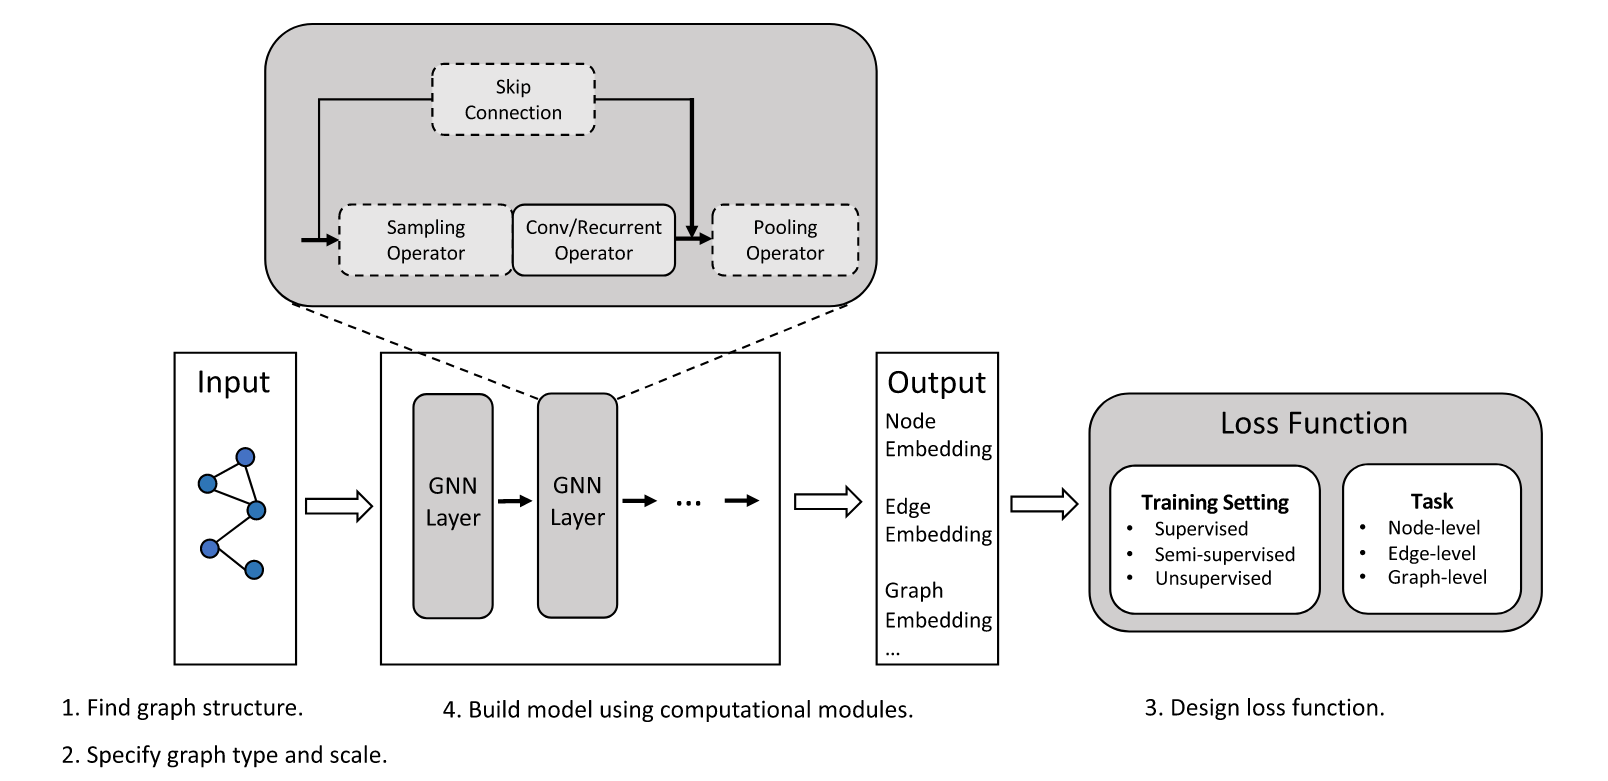
\includegraphics[width=1.0\linewidth]{graphics/GNN-pipeline.png}
    \caption{Overview over a GNN training pipeline \cite{gnn_overview}}
    \label{fig:GNN-pipeline}
\end{figure}

A classical example for a GNN is the GCN, the Graph Convolutional Neural Network. Convolution is a very broadly used operation in a wide variety of ML tasks, such as Image Processing. It uses a computationally performant approximation to spectral graph convolutions, which are a generalization of convolutions from images or audio. The propagation that is performed then follows the following formula:
$$H^{(n+1)}= \sigma(\tilde{D}^{-\frac{1}{2}}\tilde{A}\tilde{D}^{-\frac{1}{2}}H^{(n)}W^{n})$$
Here the values for all node embeddings can be computed at once as the aggregation is already encoded in the adjacency matrix with self loops $\tilde{A}$, the diagonal matrices $\tilde{D}$ contain the degree of each node and $W^n$ is a weight matrix with learnable parameters (that can differ depending on the layer).\cite{gcn_origin}

Most GNN models behave similar to GCNs in the fact that they are inherently transductive and could only work with fixed graph(s). Although there have been proposals to modify them to function in an inductive setting it usually involves complex and expensive recomputations of gradients. The paper \textit{Inductive Representation Learning on Large Graphs} by Hamilton, Ying et Leskovec introduced GraphSAGE, a framework to generalize GNNs to an inductive setting. The crucial observations to their approach was to realize that a GNN with $n$ layers only uses the $n$-hop neighborhood of any node for it's final embedding. The second observation is that for most applications, $n$ stays fairly small, often $\leq 5$. That makes it technically feasible to only load the $n$-hop neighborhood as a single batch and compute the embeddings. However, an issue that quickly arises from this are ''hub-nodes'', nodes that are connected to a particularly large number of nodes. If one hub-node is part of this batch, the size of the $n$-hop neighborhood explodes. This necessitates another addition in the new sampling method, where the number of nodes that are incorporated are limited. This is achieved by performing a random draw of (at most) $k$ nodes from every nodes neighborhood, thereby eliminating the chance for a batch to suddenly blow up in size. This new method of batching the graph is dubbed Neighborhood sampling. Together with this new sampling method, three different model types were introduced, differing by the method of aggregation: \textit{Mean} aggregation, \textit{LSTM} aggregation and \textit{pooling} aggregation. The mean aggregator first takes the mean over the embeddings of all neighboring node embeddings and the target, followed by a linear transformation and finally a non-linearity function. The LSTM aggregator feeds the node embeddings into an LSTM in a random order (to guarantee independence of ordering), which still lets the model benefit from an LSTMs large expressiveness. Finally, the pooling aggregator simply applys the linear and non-linear transformations from the mean aggregator to each node individually and then takes the element-wise maximum over all resulting embeddings. 

All of these GraphSAGE variants can be trained in an unsupervised setting using standard stochastic gradient descent with this proposed neighborhood batching. The training objective is based on the shape of the graph, where nodes that are within a distance via random walk should have similar embeddings. Together with some negative sampling from the graph that enforces not-so-close nodes to be ''further'' apart.






\chapter{Methodology} \label{chap:methodology}
In this section we will first describe the approach that makes up the Contextualized Semantic Search, followed by a detailed description of the architecture and pipeline constructed to aid in training, iterating and serving webrequests for different versions of the system.

\section{Contextualized Semantic Search}
Using the established prerequisites, let's define a problem based on the data and requirements by qibri and (hopefully) solve it using the introduced techniques.

The input to our problem is a tri-partite graph with hetergenous textual metadata attached to the nodes which are in turn connected by different types of edges. One partition represents the documents in the system, one partition represents the users - authors, standard employees, supervisors, etc. - and finally the company taxonomy, how they are structured, what fields of interest the have defined, etc. The challenge is, when given a query consisting of a string, a user, or a combination of both, to find an ordering of (a subset of) the documents by how well they match the query.

Too accomplish that, we will start by producing textual embeddings for every node. These textual embeddings will be our initial feature vectors before the GNN pass. This is supposed to ensure that query strings embedded using the same encoder model stay within the ''same'' domain, so that the similarity metrics still matter. For this thesis, a pretrained BERT model was used as it required the least computational overhead to obtain the embeddings and there are many available, even for specific languages like german, which the data set of qibri is exclusively comprised of. For future work Word2Vec might be worth testing, as it is one of the more easy models to train and As for the similarity metric, cosine similarity was used, since it is one of the most common and well supported similarity mechanisms by most vector databases and length information doesn't matter thereby disregarding potential scaling issues which result after the application of the GNN. To obtain the GraphSAGE model, a training loop with hyper parameter optimization was created. The loss function of the training loop was the unsupervised setup described in the paper, combined with an L2-loss to keep the contextualized embeddings as close to the inital embeddings as possible. For the choice of the hyper-parameters, the similarity between each initial and final node embedding was computed and averaged, as well as testing if certain edges that were not present in the training set were there, namely favorite information between users and documents.

\section{Architecture}
The system is completely contained to run within a docker container with two separate entry points. Firstly, there is a webserver defined via FastAPI with which the Knowledge Graph can be queried. This includes basic semantic search and the contextualized semantic search, the later also including a naive user-based relevance (using the mean between the two embeddings). Additionally, logical filtering to assert documents are linked to certain departments, users, etc. can be applied to the search query. This webserver is intended to run as a separate microservice within a Kubernetes environment.
The second entrypoint is running the pipeline, which will be described in detail in the next section. However, for the sake of completeness, the interfaces to other services will be briefly described from a birds eye view. Figure \ref{fig:quaesitum-arch} illustrates this: In the top section, the three distinct storage entities are displayed. The Graph \& Embeddding datastore, which in this case is a simple sqlite file, holds the Knowledge Graph in a simple nodes and edges table structure. The nodes  contain two special columns in addition to their extracted metadata. That is, the initial semantic embedding produced by the encoder model and the contextualized embeddings after the GNN pass. Furthermore, the sqlite file is checked into a git repository, with the sql dumps being versioned. This enables easy comparisons between two runs of the pipeline to see what data changed. The Document Storage and the Document Content Storage both are simple directories on the container that can be mounted for caching. The difference between the two is, that the Document Storage contains plain file downloads from qibri - which means it could also simply be hooked to a remote storage like an S3 bucket and thereby save time and ressources by not having to download all files via the api. Meanwhile, the Document Content Storage contains the results from an external service, chunkr \footnote{https://chunkr.ai/}, which extracts the contents of a file using a mixture of file parsing and ocr.


\begin{figure}
    \centering
    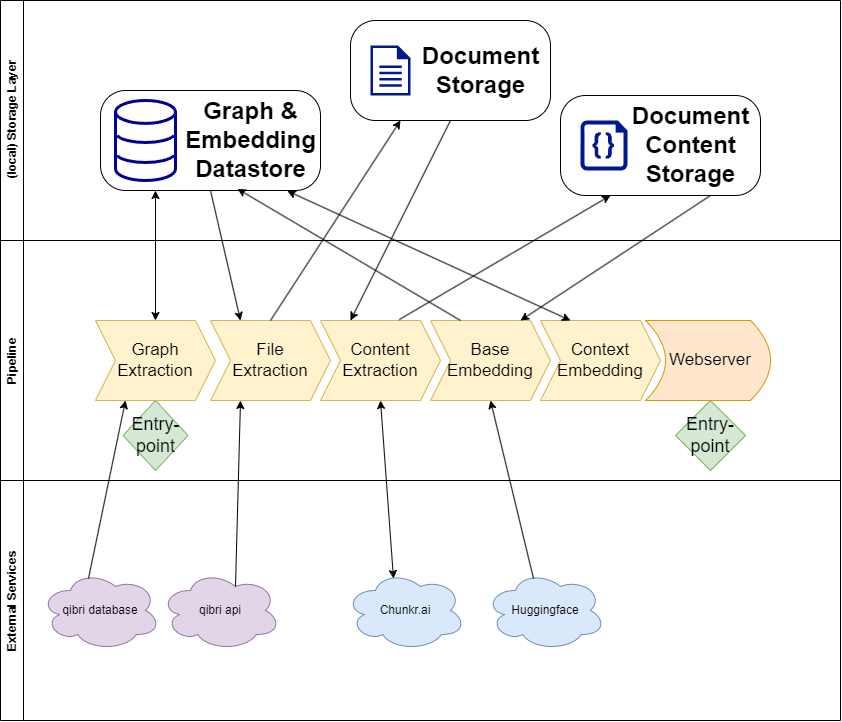
\includegraphics[width=1.0\linewidth]{graphics/quaesitum-arch.png}
    \caption{A birds eye view over the quaesitum architecture. The top row displays all storage entities used }
    \label{fig:quaesitum-arch}
\end{figure}

 
%\section{Practical Considerations}
%The code in the repository can be split into two distinct parts. The embedding pipeline, which was the main focus, and the webserver providing the search functionality.The main technologies used for this thesis were python with several important libraries, to provide the necessary functionality, and docker, for ease of development and deployment. The main packages used were pytorch and pytorch\_geometric, for the GNN training, sentence transformers, which is a package provided by Huggingface, an online hub for publicizing open source models and was used for obtaining the initial embedding model, and fastAPI, which is a python library meant to quickly set up a webserver.The embedding model that was used is a Bert model by the Deutsche Telekom company, which was published to Huggingface. \cite{german_bert} The aim of this section is to provide a more in-depth description of the practical aspects of this thesis and the considerations with which they were developed as well as how they were accomodated.

\section{Pipeline}
The pipeline can be broadly split into content extraction \& graph creation and embedding \& contextualization. The content extraction starts by connecting to the qibri database and fetching the latest published versions of all documents and document collections (so-called guidelines), all users and the taxonomy, as well as all links between these entities. This information is used to construct the actual Knowledge Graph. Furthermore, the files for every document entity need to be fetched. This can be done in two different ways, either by externally mounting the Document Storage to the container as mentioned previously or by directly accessing the qibri api. After this step is done, the documents are sent to chunkr, which extracts html and markdown representations to be used in the next step. 

After the extraction is finished, the embedding process begins. For the base embeddings, every entity is retrieved with their entire textual content associated and fed into the textual embedding model. As of right now the model is a german BERT variant, labeled ''deutsche-telekom/gbert-large-paraphrase-cosine'' on huggingface, published by the Deutsche Telekom.\cite{german_bert} This model was chosen because the embedded texts are german corporate documents and this model seemed to be trained on the most similar data. The text was then embedded without further processing or finetuning of the model, since first tests where the initial embeddings where used for a basic Semantic search seemed to indicate that enough meaning of the documents were recognized to for further processing. Additionally, since one of the goals was to see if the GNN would improve the representations, the data was left as is. 

For the Content Embedding, a GraphSAGE model was fit using a hyper-parameter optimization framework, optuna \footnote{https://optuna.org/}. The initial features of the nodes were the aforementioned base embeddings and for the links all edges in the  Knowledge Graph were used - apart for some ''favorite'' edges between users and documents, which were used as a validation set.  The training used a semi-supervised loss function which was a binary cross entropy loss over the initial edges with negative sampling, as it was proposed in the paper as a completely unsupervised method. Additionally, a L2 loss was used to try to constrain the model to stay as close to the inital embeddings as possible. For the validation task the model was tasked to predict favorite edges between users and documents/guidelines, which were not present in the training set. Additionally, the cosine similarity between a the initial text embeddings and the node embeddings after the GNN pass was used in order to ensure that the resulting embeddings were as close to the initial embeddings as possible. 

Finally, at the end of the pipeline, the model and the embeddings were saved. Both the Knowledge Graph and the embeddings are stored in the sqlite file. Sqlite was chosen because it is easy to create, destroy and replicate databases, it has a vector extension (sqlite-vec) that makes it possible to run vector comparisons easily, while staying lightweight and performant through the fact that it is embedded into the process. To keep track of the different iterations, the database is checked into a git repository and iterations of the database are kept track of in snapshots.


\section{Notes on Implementation}
The whole project was intended to be used completely autonomously within qibri's kubernetes cluster. For this purpose, a container image was defined to accomodate both the pipeline and webserver. To ensure clean horizontal scaling, all webserver instances are sessionless and read-only so that the same sqlite file can be replicated across any number of webservers. To spin up another instance, all secrets have to be passed to the container via environment variables, then the sqlite file has to be made accessible to the container (either via a shared volume, or by straight-up copying the database into the new container). Additionally, every customer has a separate pod dedicated to them, thereby enabling per-customer scaling where the load of users of one customer don't affect another. 
Finally, to enable auto-deployment, the containers are automatically built via github actions and pushed to a container repository to make deploying new versions a seemless experience.
%\section{Architecture and Code}
%The search is built as a standalone docker container with all secrets passed via an env file. The results are written to an external volume specified in the docker-compose file, where an sqlite3 file contains the knowledge graph and all node embeddings, while a subfolder contains all files downloaded from the qibri backend and, where possible, an additional file containing the extracted content using Chunkr \footnote{An external service for extracting text from a variety of files \url{https://chunkr.ai/}}. The sqlite3 database is checked into a separate git repository to make it possible to go to a specific run of the pipeline and compare results.

%There are two different entry points for the program. One is a webserver, to provide the actual search as a microservice. The second is the pipeline, which starts a fresh extraction of the Knowledge Graph of a specific customer from qibri, writes that to the SQLite file (after dropping it), downloads potentially missing files, runs the GNN training loop and finally writes the obtained embeddings to the SQLite file as well, thereby providing the vectors used by the search in the webserver.





\chapter{Discussion and Improvements} \label{chap:discussion}
As of writing this thesis, the proposed search engine has not been able to be properly tested, because there was no good way to validate it without letting users test it, which in turn was not possible without integrating it into the application. This is currently under way and analytics from user interactions will be collected both for evaluation and more fine-grade training.

Nevertheless, some details are already quite clear. The extraction process from qibri has proved resilient to minor changes and adjustments, storing the data in an sqlite database has had no noteworthy drawbacks while retaining all discussed benefits of such a light-weight datastore. The webserver also seems to have served it's purpose well for the time being, with no glaring delays in serving requests, even when considering pythons infamous snail's pace. In addition, the fact that the service can be scaled and replicated so easily also suggests that performance won't be an issue. 

As indicated before, the system still is in no state for testing - Although the base embeddings of the search engine without the GNN pass seemed to represent the domain reasonably well, incorporating user embeddings to obtain joint embeddings did not yield any satisfactory results. After the GNN was applied, even the basic semantic search with only a query string seemed broken. Query results had no clear order and out of the top ten results at most one or two had any remote relevance to the query. Searches that had provided reasonable results prior to the graph contextualization no longer returned results that could be considered ''decent'' by any means. \\
After some investigation, it seems that although the expected results still have a decently high similarity score, a lot of false positive results have the same or higher scores, thereby messing up the performance. \\
This could indicate a too small amount of negative sampling, which would encouraging false positives through a too high degree of smoothing, which seems to be a common issue for GNNs. 

For the user-based recommendations and combined searches of users plus query string, there are several additional error sources that may also come into play, most of them due to lacking data. Most importantly: There is little to no data available on the users themselves. That is, the user embeddings are generated essentially only on the name of the user themselves. This is necessary, since there has to be some initial embedding to start from and random embeddings aren't possible, since the text embedding of a users name should also be related to their node embedding. This is so that documents that mention a user by name might get a notion of similarity to the user node in the graph from this name appearing, without any additional connections via e.g. authorship. An unwanted side-effect, however, are the unwanted similarities through speaking names, e.g. Forster (similar to Förster, german for forest ranger) having a high similarity to documents related to wood, paper, etc. Let it be know that this is meant as an illustratory example, not an actual occurence. Nonetheless, these problems would probably also be mitigated by more data to embed on individual users. \\
For the joint queries with a query string and a user, the limited time didn't really allow a deep finetuning here. For now, the two embeddings (the node and the text embeddings) were added together and that was used as the basis for the similarity search. Here especially the bootstrap dilemma of needing a model to get feedback but needing feedback to train a model strikes especially hard. For more sophisticated techniques to be used, data about user preferences would be necessary, However, the only real data that is available at this time and that can be used for this purpose is favored documents by users, but in the entire document corpus about 2 percent are favored, which are favored by an equally small fraction of users. 

%An interesting finding that was discovered at the end of this thesis is the fact that the implementation of GraphSAGE used in PyTorch-Geometric seems to treat \textit{all} node embeddings, including the one of the current node the same and aggregates them - which means the model \textbf{can not} learn biases towards it. This is highly problematic as the wanted target embedding should be very close to the initial embedding with the aggregated neighborhood embeddings only ''nudging'' the embedding in another direction. An approach that the paper mentions concatenates both embeddings together before applying a linear transformation and afterwards another nonlinearity function. 
%An alternative would be to take a page from the transformer architecture, which adds every the input and output to every Multi-Head Attention layer together and normalizes it, before feeding it into the next layer. if this multiplication is scaled additionally by a learnable parameter, this should also come close to the idea of nudging.

\chapter{Conclusion and Future Work} \label{chap:conclusion}
The primary goal of this thesis was to design, implement, and initiate testing of a framework that enables semantic search enhanced by Knowledge Graph-based contextualization. The work focused on building an end-to-end pipeline that could extract relevant graph structures, train a semantic representation model incorporating neighborhood information, and deploy a search engine capable of serving real-time queries within a production environment.

The entire framework was implemented in Python and leverages several key technologies, including PyTorch Geometric for graph processing, Sentence Transformers for text embeddings, FastAPI for serving API requests, and SQLite for lightweight persistent storage. Containerization using Docker ensures that the system is portable and easily replicable, allowing for straightforward horizontal scaling to meet the demands of concurrent users.

The current version of the framework has been successfully built and is in the final stages of preparation for deployment within the qibri application ecosystem. Initial testing has confirmed the viability of the approach but has also revealed several limitations in the contextualization mechanism. In particular, the integration of Knowledge Graph structure into the semantic search process — while conceptually sound — requires more data and further refinement to deliver meaningful performance improvements in real-world scenarios.

In summary, this thesis provides a solid foundation for deploying semantic search systems that integrate structured knowledge. While the core infrastructure is complete and operational, achieving high-quality, domain-sensitive retrieval remains an open challenge that invites further exploration.

\section{Future Work}
The most important open topic would be the finetuning of the GNN aspect. This involves testing more hyper parameters and performing further experiments with potentially models and methods, as this is currently barely functioning. Additionally, incorporating user feedback would be greatly benefitial to this system, as it would make an essentially unsupervised task into a semi-supervised one, which could alleviate a lot of the difficulties. 

Another improvement with a lot of potential would be online, local updates. The graph structure within qibri is not static - some areas, e.g. the documents, see frequent updates, while others, e.g the taxonomy structure, remain largely the same over long periods of time. This means that it shouldn't be necessary to re-embed the entire graph every time something changes, but to update only the affected nodes. One of the main reasons for using GraphSAGE with the neigbhorhood sampler was in order to enable incremental updates of the contextual embeddings later on. To solve this, all information needs to be timestamped in order to keep track of new information and diffs between the existing graph structure in the index and the newly extracted ones need to be computed.

Additionally, update strategies for different types of changes need to be investigated. A completely separate idea that might be worth considering in general is a hybrid search - using a classic full-text search together with a sematic search and calculating a joint ranking between the two. This might cover current blank spots such as partial strings which a lot of people still use when searching for specific documents.



\backmatter

% Declare the use of AI tools as mentioned in the statement of originality.
% Use either the English aitools or the German kitools.
\begin{aitools}
This thesis benefited from the use of AI tools in specific areas. ChatGPT was employed to rephrase and polish sections of the abstract and conclusion. Gemini was used for similar rephrasing and polishing tasks, except that it was limited to the refinement of this declaration. For grammatical and lexical checking, the writeful integration of overleaf was employed (until the free tier expired), as well as the browser extension Languagetool.
\end{aitools}

\begin{kitools}
Diese Arbeit profitierte in bestimmten Bereichen vom Einsatz von KI-Tools. ChatGPT wurde verwendet, um Teile des Abstracts und des Fazits umzuformulieren und zu überarbeiten. Gemini kam für ähnliche Umformulierungs- und Überarbeitungsaufgaben zum Einsatz, beschränkte sich jedoch auf die Verfeinerung dieser Erklärung selbst. Für die grammatikalische und lexikalische Überprüfung wurden die Writeful-Integration in Overleaf (bis zum Ablauf des kostenlosen Zugangs) sowie die Browser-Erweiterung LanguageTool genutzt.
\end{kitools}

% Use an optional list of figures.
\listoffigures % Starred version, i.e., \listoffigures*, removes the toc entry.

% Use an optional list of tables.
\cleardoublepage % Start list of tables on the next empty right hand page.
\listoftables % Starred version, i.e., \listoftables*, removes the toc entry.

% Use an optional list of alogrithms.
%\listofalgorithms
%\addcontentsline{toc}{chapter}{List of Algorithms}

% Add an index.
\printindex

% Add a glossary.
\printglossaries

% Add a bibliography.
\bibliographystyle{alpha}
\bibliography{intro}

\end{document}
